\chapter{Casistica, materiali e metodi}

\section{Casistica}

Introduzione alle informazioni della mostrate

\subsection{Paziente 1} % Ma.Va.

Breve descrizione ...

\begin{table}
\begin{tabular}{ll ll}
\toprule
\multicolumn{4}{l}{\textbf{Dati alla nascita}}\\
Luogo 		& Torino 	& Data 					& 28/12/89 (89.989)\\
Sesso 		& Femmina 	& Età gestazionale 		& 40 sett.\\
Lunghezza 	& 45 cm 	& Circonferenza cranica	& 35 cm\\
Peso 		& 3350 g\\
\midrule
\multicolumn{4}{l}{\textbf{Statura dei genitori}}\\
Padre 		& 165.5 cm 	& Madre 				& 164.2 cm \\
MPH 		& ?? \\
\midrule
\multicolumn{4}{l}{\textbf{Trattamento con GH}} \\
Età	iniziale	& ?? 		& Altezza iniziale 				& 135.5 cm  \\
Peso iniziale	& 25.4 kg	& Velocità di crescita iniziale & 4.13 cm/aa\\
Dose media		& ?? 		& Anni prepuberali trattati		& ??\\
Anni di terapia & ??\\
\midrule
\multicolumn{4}{l}{\textbf{Esito della terapia}} \\
Altezza finale	& ?? cm (?? SDS) & SDS guadagnate 			& ??\\
SDS per MPH		& ??			 & SDS guadagnate per MPH	& ??
\bottomrule
\end{tabular}
\end{table}

\section{Materiali e metodi}

\subsection{Valutazione auxologica}

\begin{figure}[h]
  \begin{center}
      \includegraphics{grafici/centili/centili.eps} %\\
  \end{center}
  \caption{Standard antropometrici neonatali relativi a peso ed altezza nell'Italia nord-orientale}
\end{figure}

\begin{figure}[h]
  \begin{center}
	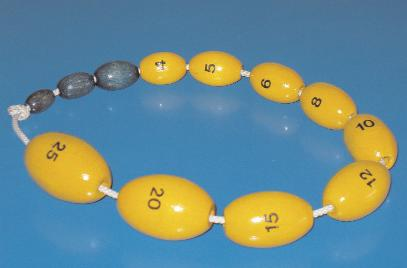
\includegraphics[scale=0.75]{grafici/orchidometro.jpg}
  \end{center}
  \caption{Orchidometro di Prader}
\end{figure}

\begin{figure}[h]
  \begin{center}
	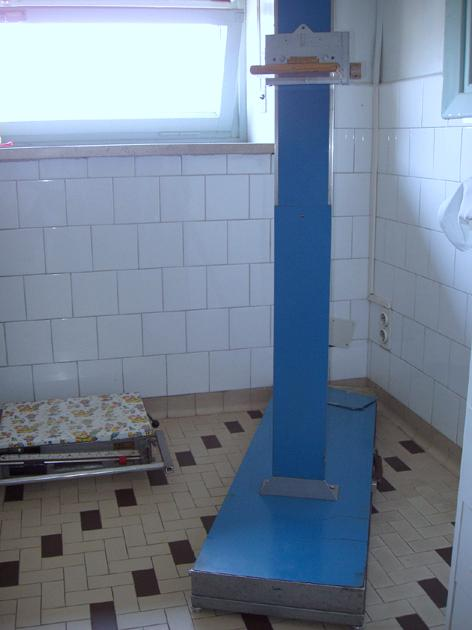
\includegraphics[scale=0.50]{grafici/statimetro.jpg}
  \end{center}
  \caption{Statimetro di Harpenden}
\end{figure}

\subsection{Valutazione ormonale}

\subsection{Analisi statistiche}
